\documentclass[journal]{IEEEtran}
\usepackage{blindtext}
\usepackage{graphicx}
\usepackage{url}
\usepackage{amsmath,amssymb}
\usepackage{float}
\setlength{\parindent}{0em}
\setlength{\parskip}{0.4em}

\begin{document}
\title{Click-Through Rate Prediction for Sponsored Search Advertising in Microsofts Bing Search Engine}
\author{Craig Heptinstall Crh13- 110005643 \\
SEM6120\\Institute of Computer Science\\Aberystywth University}

\maketitle


\begin{abstract}
In 2009, a paper by Thor Graepel \cite{bing-paper} described a winning click-through rate (CTR) prediction algorithm used for sponsored search in Microsoft's Bing search engine (the authors named this adPredictor). The paper introduced a Bayesian online learning concept that was chosen to replace the previous CTR algorithm. Here this paper looks at the concepts used in the adPredictor algorithm and how appropriate certain aspects of the task were identified and dealt with. Following an evaluation of the algorithm and paper itself, there are of course, always further improvements possible to any algorithm. Using other research, suggestions have been presented to increase the efficiency of the solution, especially over the web (since this algorithm should work efficiently during real time searches).

\end{abstract}

\section{Sponsored search}
Sponsored search is considered as one of the most profitable business models today, and according to several sources of analytic services such as analytics-magazine \cite{business-model} the four top search engines(Bing, Google, Yahoo and Baidu) make in excel of \$37 billion. Bing however gets the lion share with over \$25 billion of the total coming its own way. Therefore, keeping this amount on an upward trend requires appropriate and efficient advertisements. \par
Sponsored search uses two key aspects to the use of a search engine that can be applied to providing advertisements:
\begin{itemize}
\item The query the users enter- This indicates the requirement of the user
\item Users clicking on advertisements- This gives users the opportunity to see advertiser's pages
\end{itemize}
In order to get the advertisements that is useful to the search engine (in terms of revenue), the advertisers (in terms of clicks on their links), and user's needs (In terms of relevant adverts), CTR prediction is a most vital part of a search engine.

\subsection{Click rate prediction}
The paper begins by detailing what click rate prediction is and how it fits into the web framework that is the Bing search engine. Getting an accurate metric for where advertisements will be clicked is important to the user, and more so the search engine. By being able to get the probability of an advert being clicked, the authors are able to increase further the possible profitability of the search engine via advert placement, and assisting the choice of adverts to be displayed. \par
Although the paper describes CTR well as a starting point, the graph in figure \ref{fig:CTR} shows an example of how keywords and where they are placed on a page affect the CTR. By having a good predictor, the keywords and placement of adverts will be more informed before they are added to search.

\begin{figure}[!ht]
  \caption{CTR based on position of advertisement. Image taken from a marketing explanation of CTR \cite{ctr-image}.}
  \centering
  \label{fig:CTR}
    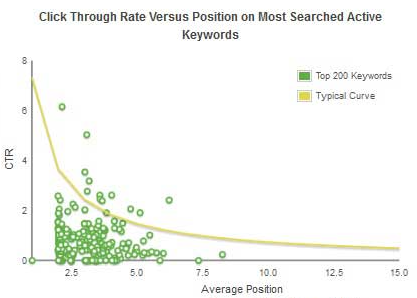
\includegraphics[width=0.5\textwidth]{CTR}
\end{figure}

\subsection{Keywords auction}
In order to grasp the whole concept of CTR prediction, keyword auction is something that the paper describes as an important feature in displaying advertisements in their specific places. Rather than having selected ads chosen by the selecting algorithm just place them in any order on the screen, keyword auction uses an algorithm known as generalized second price (GSP). This ensures that advertisers pay appropriate amounts referring to what position they appear on a search page. \par
GSP is a fairly simple algorithm \cite{keyword-auction}, which takes in a number of bids from bidders (in this case advertisers) all of which specify amounts they are willing to pay for clicks on adverts related to certain keywords. Following the auction, the bids with the highest prices win the best place, but only pay the second highest bid price. After this, the second highest pays the second highest bid and so on. Predicting which advertisements will be used by users heavily relies on the results from a GSP, which the adPredictor paper expands on with constraints that this way of generating advertisements brings.

\section{Challenges approached by adPredictor}
There were a number of existing problems that needed to be solved by any CTR predictor in order to create an efficient solution that would be enough to replace Bing's previous predictor. These range from getting suitable input features for the predictor, to evaluating the performance of the predictor itself. This section of the paper looks at each of these in relation to what the adPredictor authors had to accomplish in order for their solution to work.

\subsection{Features and impressions}
With any machine learning algorithm, there must be appropriate input features that can represent variables used to produce outcomes (in this case binary). Because the web is quite diverse, and is forever changing, many different aspects of a user's actions should be considered when predicting click through rates. The authors of adPredictor questions the availability of inputs, and comes to a conclusion that at least three main categories should be considered when attempting to create the probability of a user's click:
\begin{enumerate}
\item Ad features- The adverts themselves, including links, text on the adverts and the campaign of the ad.
\item Query features- These are directly entered by the user, such as words searched by the user.
\item Context features- Indirectly given by the user, to personalise adverts more. These could be the location of the user, time and date to name a few.
\end{enumerate}
Because of the vast size features possible, the complexity of the algorithm had to be considered, alongside the speed of which the predictor would function. Selecting good features is one of the building blocks of any machine learning algorithm. In a lecture by Jeff Howbert at Washington University \cite{washington}, he mentions the 'Curse of dimensionality' and states that as features increase the volume of feature space increases too. This makes data harder to understand and results in an increase of difficulty of achieving statistical significances.

\subsection{Isolated predictions}
The next task challenging the authors was the testing of the predictor. In order to actually see results from their algorithm, there was the task of seeing how well it performed. Although the author suggests a number of ways that machine learning predictors can be tested (AUC (area under the receiver operator curve), or log-likelihood of test data), with the predictor being part of a larger system means that different goals from users, advertisers and the search engine may conflict resulting in inaccurate test results.

\subsection{Dynamic web}
Another challenge identified in the paper looks at the dynamic behaviour of the web. Because the web is not a static object, the ways people use it will vary over time. The authors also highlight such times as seasonal changes, changes in viral interest and economic behaviours that can all change the way the general interest of different searches head. Following this, the CTR predictor must be able to cope with changes in clicks for certain topics. Because the current ad-selection technique (keyword auction) only bases its choices from advertisers who will update their target markets, it means that long term click through rates will be ignored, whilst the algorithm used in a predictor would still be trying to base its predictions from learning with older data.

\subsection{Computational issues}
A final issue identified by the authors, and generally across wide research into CTR predictors is the worry of computational power. With the scale of the web being so large, the amount of advertisements and their data can be extremely large. With each search having to calculate and bring back the most appropriate advertisements almost instantaneously, the algorithm defined in the resulting paper had to be as efficient as possible. \par
Training of the algorithm must also be performed as quickly as possible to keep up with the changing trends of a web platform. There is a trade-off between accuracy and computing time that had to be considered. A paper that looked at a similar system created for Facebook advertisements \cite{facebook} highlights the importance of 'keeping memory and latency contained for massive scale'. The creators of adPredictor would also have had to ensure that as much data could be used as features, while keeping the speed of the predictor at a sufficient level.

\section{adPredictor solution}
For the solution presented in the paper, the authors chose to start with a general Bayesian online learning algorithm, and then mutated this to work with CTR terminology. The image below \ref{fig:bayes} indicates the general use Of Bayes rule, where in this case the posterior being the binary outcome of whether the user would or would not click the advertisement. \par

\begin{figure}[!ht]
  \caption{General Bayes rule, where \(P(h \mid d)\) is the binary probability of clicking an advertisement}
  \centering
  \label{fig:bayes}
    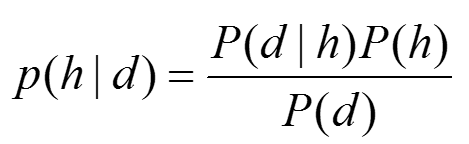
\includegraphics[width=0.3\textwidth]{bayes}
\end{figure}

The algorithm bases itself off a probit regression model that takes in features (in this case the three categories mentioned earlier: ad, query and context features), and performs online Gaussian updates to the model created. Continuing from that to suit it more towards the use of online CTR prediction, pruning of some common features are performed to cut the training time of the algorithm. Finally, the algorithm uses parallel training to ensure that new data from the ever-changing web are taken into account, avoiding solely building on already existing static data. \par
Notating the outputs of the algorithm was the first step in the adPredictor algorithm, and the authors made it so a simple vector would hold a range of feature values for an advertisement, and where the outcome of a click/ none click will be represented by 1 or -1 for notational convenience. 
The probability model the authors decided to use was a generalised linear model with a probit link function. From comparison of this with a standard linear model, there could be two reasons for this use (both of which can be also explained in textbook found about GLM's from Dell \cite{dell}):
\begin{enumerate}
\item Distribution of dependent variable- The dependent variable (in this case click rates) may not be continuous in a linear distribution.
\item None-linear effect of prediction- The effect of the predictor will not be linear, because the nature of clicks by users will not be concrete.
\end{enumerate}
At this point, Gaussian prior distribution is applied over the weights of the model, in order to take into account previous click estimations. The paper represents this in a factor graph model, showing how the probit regression function works. The model takes in Gaussian prior weights, calculates a score for each, and then compares a zero-mean Gaussian of the weight with a given threshold. \par
The paper talks about the use of 'update equations' which allow the algorithm to become more a natural online learning means, taking into account any prior information (such as historical average CTR). The possible issue here (as mentioned in section 2.C) is that with the dynamics of the web, historical averages may not be sufficient in the learning of the algorithm. \par
Continuing on with the need for a solution to web dynamics, the algorithm then puts in place a model of dynamics that converges back to the prior rather than to a uniform distribution of weights. By delaying updates of weights, computationally it makes it possible to apply updates cumulatively resulting in the allowance of new data. \par
Another important aspect of the solution proposed in the paper looks more towards the computational costs of the algorithm when placing it in a web environment. As identified in the potential issues from the previous section, the memory and data size footprint must be limited in order to allow this algorithm to be deployed for its intended function. By compressing the model to only concentrate on features that appear commonly (though new features should be considered in case they become a new common), the model will not waste memory on them. \par
Training and feedback of the usefulness of the algorithm was a potential issue that the authors had to address. The paper states that because it is based on an online learning algorithm, usually training is performed from previous iterations. With the dynamics of the web, this is problematic. In order to solve this issue, parallel training is used in order to avoid each training procedure being taken in turn. By using a distributed factor graph, each training example can be scheduled to run as effectively as possible. In a paper by Xufeng Han about a similar use of parallel training \cite{training}, they support the avoidance of single machine methods that tie together all parameters which are computationally expensive. \par
The paper went into some detail about the results found from their proposed solution, and used a Niave Bayes algorithm to compare with. As this was one of the more commonly used algorithms at the time, this was an ideal method to test against. By comparing the ogarthmic loss of both, the graph produced could show the probability of click for a set of advertisements. The graph in figure \ref{fig:results} showed that the newer adPredictor was generally more accurate.
\begin{figure}[!ht]
  \caption{Histogram over impressions of predicted probabilities, showing authors' algorithm making more spread out and informed decisions.}
  \centering
  \label{fig:results}
    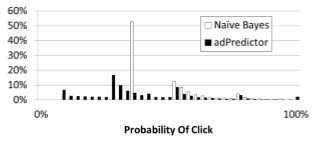
\includegraphics[width=0.5\textwidth]{results}
\end{figure}

\subsection{Solution issues}
Following the explanation and evaluation of various stages in the creation of the adPredictor algorithm, there a few issues have been identified, which may be improved on in the future, some of which improvements will be considered in the following section. It is hoped that each of the solutions provided for these issues could be combined into one hybrid approach that should perform better than the previous. \par
These are as follows:
\begin{itemize}
\item Web dynamics- incorporated new data from the dynamic web is not considered enough.
\item Training data used- Currently, the paper states that CTRs are usually lower than 50\%, which means a lot of the data and features used to retrain the algorithm is waste in terms of training time.
\item One paper \cite{lasso} which talks about a complete different means of CTR prediction states that logic regression models make it difficult to capture nonlinear information from user features and ad features, which could be important when wanting to use this conjunction information to know that for instance "people with more buying power should be interested in luxury products".
\end{itemize}
Starting with the first issue identified above, this looks at issue of the algorithm working with a currently very active web. Although the algorithm looks at using previous learning experiences to increase its efficiency in future predictions, the way it handles new data from a dynamic internet is not in-depth enough. \par
This issue also extends to the actual testing of the algorithm. In the paper which looked at Facebook's own ad prediction algorithm \cite{facebook}, the author mentions that because click prediction systems are usually deployed in dynamic environments, that having tested the same data model over consecutive days without retraining it, that they saw the accuracy cleared degrade for the CTR predictor. If the author of the Bing ad predictor had tested this way, they could have found out the most appropriate length of time between needing to retrain the model. \par
The next potential issue found looks at what training data is used. One paper, by H. Brendan, talks about sub sampling data in a section about saving memory at in a web scale algorithm. The way the current algorithm works means that more than just clicks are taken into account when retraining for the next iteration of running. This could indeed slow down over time, as more and more unique features are identified. Even with the use of the parallel training explained earlier, the time taken to compute each weight variable will always be more when more features are taken into account. \par

\section{Suggested alternatives}
Following the reported possible issues found from reading the solution provided in the adPredictor paper \cite{bing-paper}, there are some alternatives and improvements to the concepts in the algorithm. Although the brief of this paper was to suggest a better machine learning approach to the one already provided, it is hoped that by combining the aspects of the following suggestions could come together to produce an overall better solution. \par
The first of which looks towards the ‘data freshness that was discussed around the need to update the model regularly. As mentioned in the Facebook paper \cite{facebook}, by testing with some static data that the model was trained on over a few consecutive days, it would be possible to calculate the most efficient amount of time to retrain, before losing too much accuracy. In the Facebook example, they found that retraining daily was the best option for their own LR model, although some concern should be shown where data amounts mean that retraining may take longer than 24 hours to complete meaning a daily retain would not be possible. \par
The next proposed alternative deals with the second issue, which could be solved by sub sampling the data used to train the algorithm. In the paper exploring various current challenges of CTR predicting \cite{trenches}, the suggestion is made to only reduce data training size and only concentrate on two sub samples:
\begin{enumerate}
\item Queries where at least one ad was clicked
\item A fraction of queries where no ads were clicked
\end{enumerate}
By doing this, the sample of training data is cut tremendously, meaning the speed at which it can train and search is greatly improved. The paper also suggests how to avoid biased decisions because of the naive training. In figure \ref{fig:importance}, importance weights can be assigned to ensure fairer sets of data.
\begin{figure}[!ht]
  \caption{Weight importance, where t is in a clicked query, and where t is in a query with no clicks.}
  \centering
  \label{fig:importance}
    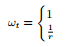
\includegraphics[width=0.08\textwidth]{importance}
\end{figure}
The final change, though more drastic that the previous two that could be implemented in a hybrid approach to improve the machine learning solution could be to change the entire model used. Rather than the LR model used, a model called CGL (Coupled group lasso) would bring in some advantages such as fixing the issue with conjunction information, where user's features would be linked to the features of the advertisements. CGL also eliminates useless features, which is what is trying to be achieved with the previous improvement.\par
CGL is a relatively new model type, and has not been widely used, but in the paper suggesting the use of it for CTR prediction by Lin Yan \cite{lasso} says it has a greater accuracy of prediction than a traditional LR based predictor. To support this, the paper includes a figure \ref{fig:improvement} which shows the difference in accuracy over LR.  
\begin{figure}[H]
  \caption{Relative improvement of CGL over LR in terms of accuracy based on three random data sets.}
  \centering
  \label{fig:improvement}
    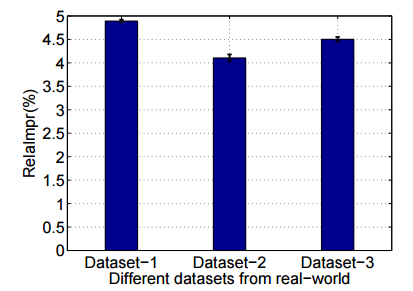
\includegraphics[width=0.5\textwidth]{graph}
\end{figure}
\par
In order to measure this, the author used a widely adopted metric known as ‘RelaImpro' meaning relative improvement. It can be considered as so:
\begin{figure}[!ht]
  \caption{The Relative improvement metric.}
  \centering
  \label{fig:relaimpro}
    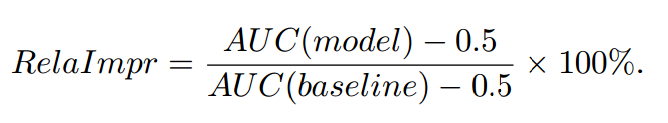
\includegraphics[width=0.5\textwidth]{relaimpro}
\end{figure}

\section{Evaluation}
Following the review of the paper, and the suggested issues and resolutions, future work can be identified. In addition to the hybrid approach suggested in this paper, there has been on going advances in both machine learning and CTR prediction specifically. As the Bing paper was published in 2009, papers holding new ideas such as Coupled Group Lasso for CTR prediction have shown that approaches such as this one will one day become less efficient in terms of what other options there may be. \par
From the viewpoint of the author, in terms of this paper and its suggestions, most ideas and concepts were kept quite high level in their descriptions in order to keep the length of the paper to a limit, therefore restricting the detail needed in order to compare the ways models, probability or training is performed in terms of the calculations used. In terms of the assignment requirements, the need to keep it basic enough for a reader to grasp concepts of machine learning has been kept a priority for this paper.

\subsection{Future developments}
With any research, there is always the possibility of future works. Identified in the original solution paper, the authors mention the exploration of alternative models, such as feature based method "Matchbox” for using more personalised data of users in order to give those more tailored ad predictions. In fact, In a recent library publishing by Microsoft, they have now persuade and implemented this predictor type in a Microsoft Azure module \cite{azure}. The predictor in the library compares the previous type of model (as used in this algorithm) and the new collaborative filtering method, stating that the second only uses identifiers of users, and obtains detailed information from a sparse matrix given by the users trending searches. \par
By learning more about an individual user, this would mean more profitable advertising, though as outlined in the first section of this report, the issue would still remain that the sheer number of individual users searching via Bing may be too large to handle such a dense amount of personalisation.

\begin{thebibliography}{1}

\bibitem{bing-paper}
T.~Graepel, \emph{Web-Scale Bayesian Click-Through Rate Prediction for Sponsored Search Advertising in Microsoft's Bing Search Engine}, \hskip 1em plus
  0.5em minus 0.4em\relax Microsoft Research Ltd, 2010.
  
\bibitem{business-model}
P.~Quinn, \emph{Sponsored search advertising}, \hskip 1em plus
  0.5em minus 0.4em\relax Analytics Magazine, \emph{\url{http://www.analytics-magazine.org/may-june-2012/580-online-analytics-sponsored-search-advertising}}, 2012.
  
\bibitem{keyword-auction}
B.~Edelman, \emph{Internet Advertising and the Generalized Second-Price Auction:
Selling Billions of Dollars Worth of Keywords}, \hskip 1em plus
  0.5em minus 0.4em\relax \url{www.benedelman.org}, 2006.
  
\bibitem{ctr-image}
L.~Kim, \emph{Five Must-Have Insights for Better PPC Campaign Performance}, \hskip 1em plus
  0.5em minus 0.4em\relax Marketing Profs, \emph{\url{http://www.marketingprofs.com/articles/2014/24562/five-must-have-insights-for-better-ppc-campaign-performance}}, 2014.
  
\bibitem{washington}
J.~Howbert, \emph{Machine Learning: Feature Creation and Selection
}, \hskip 1em plus
  0.5em minus 0.4em\relax \url{http://courses.washington.edu}, 2012.
  
\bibitem{facebook}
X.~He, \emph{Practical Lessons from Predicting Clicks on Ads at Facebook}, \hskip 1em plus
  0.5em minus 0.4em\relax \url{https://research.facebook.com/publications/practical-lessons-from-predicting-clicks-on-ads-at-facebook/}, 2014.
 
\bibitem{dell}
Dell.Inc, \emph{Generalized Linear Models}, \hskip 1em plus
  0.5em minus 0.4em\relax Marketing Profs, \emph{\url{http://documents.software.dell.com/Statistics/Textbook/Generalized-Linear-Models}}, 2015.
  
\bibitem{training}
X.~Han, \emph{DCMSVM: Distributed Parallel Training For Single-Machine Multiclass Classifiers}, \hskip 1em plus
  0.5em minus 0.4em\relax Marketing Profs, \emph{\url{http://acberg.com/papers/dcmsvm.pdf}}, 2010.
 
\bibitem{trenches}
H.~Brendan McMahan, \emph{Ad Click Prediction: a View from the Trenches
}, \hskip 1em plus
  0.5em minus 0.4em\relax Marketing Profs, \emph{\url{http://jmlr.org/proceedings/papers/v32/yan14.pdf}}, 2013.
  
\bibitem{lasso}
L.~Yan, \emph{Coupled Group Lasso for
Web-Scale CTR Prediction in Display Advertising}, \hskip 1em plus
  0.5em minus 0.4em\relax Marketing Profs, \emph{\url{https://www.eecs.tufts.edu/~dsculley/papers/ad-click-prediction.pdf}}, 2014.
  
\bibitem{azure}
Microsoft, \emph{Train Matchbox Recommender}, \hskip 1em plus
  0.5em minus 0.4em\relax Marketing Profs, \emph{\url{https://msdn.microsoft.com/en-us/library/azure/dn905987.aspx}}, 2015.
  
\end{thebibliography}

\end{document}
